\documentclass[13pt]{extarticle} 

% --- 1. Paquetes Base y Matemáticas Fundamentales ---
% (Deben ir ANTES de las fuentes)
\usepackage[utf8]{inputenc}
\usepackage[spanish]{babel}
\usepackage[margin=2.5cm]{geometry}
\usepackage{amsmath}           % Solo amsmath (newtxmath ya cubre amssymb y amsfonts)
\usepackage{mathtools}
\usepackage{physics}

% --- 2. Tipografía y Espaciado ---
% (newtxmath se carga después de amsmath para evitar el error \Bbbk)
\usepackage{newtxtext,newtxmath} 
\usepackage{setspace}            
\onehalfspacing                  

% --- 3. Utilidades Gráficas y de Formato ---
\usepackage{graphicx}
\usepackage{xcolor}
\usepackage{hyperref}
\usepackage{fancyhdr}
\usepackage{titlesec}

% --- 4. Ajuste de Párrafos ---
\setlength{\parskip}{1em}        
\setlength{\parindent}{0pt}      

\begin{document}


\begin{titlepage}
    \centering
    \vspace*{0.5cm}
    
        % Encabezado Institucional
    {\scshape\LARGE Instituto Tecnológico Autónomo de México \par}
    \vspace{1cm}

    % Logo Institucional
    
\includegraphics[width=0.45\linewidth]{Imagen soltada.png} \\[2cm]
    

    
    % Título del Proyecto
    \rule{\linewidth}{0.6mm} \\[0.5cm]
    {\huge \bfseries Análisis Dinámico Riguroso y Simulación Computacional del Péndulo Doble} \\[0.2cm]
    \rule{\linewidth}{0.6mm} \\[2.5cm]
    
    % Información del Curso y Profesor
    {\large \textbf{Asignatura:}} \\
    {\large Sistemas Dinámicos II} \\
    \vspace{1cm}
    
    {\large \textbf{Profesor:}} \\
    {\large Ernesto Pérez Chavela} \\
    \vspace{2.5cm}
    
    % Información del Alumno
    \vfill
    {\large \textbf{Presenta:}} \\
    {\large Rodrigo Moreno Cruz} \\
    \textit{Sexto Semestre}
    
    \vspace{0.5cm}
    
    % Fecha
    {\large Ciudad de México, \today}
    
\end{titlepage}

\tableofcontents
\newpage

\section*{Introducción}

El péndulo doble representa uno de los paradigmas más fascinantes de la dinámica no lineal: un sistema mecánico aparentemente simple que, bajo condiciones de conservación energética, es capaz de desplegar una riqueza topológica asombrosa y una sensibilidad extrema a las condiciones iniciales. El presente trabajo tiene como objetivo desentrañar esta complejidad, transitando desde la deducción analítica de sus leyes de movimiento hasta la visualización de su comportamiento caótico mediante herramientas de computación con python.

El análisis comienza bajo los siguientes supuestos, donde se asume masas puntuales y varillas de masa despreciable en un entorno carente de fricción. Utilizando el formalismo de la mecánica lagrangiana, se derivan las ecuaciones de Euler-Lagrange, obteniendo un sistema de segundo orden altamente acoplado. Para facilitar su estudio bajo la óptica de los sistemas dinámicos, este modelo se transforma en un campo vectorial autónomo en un espacio de fases tetradimensional ($\mathbb{R}^4$), donde se garantiza la existencia y unicidad de las trayectorias mediante la verificación de la condición local de Lipschitz.

A lo largo del desarrollo, se aplica la teoría cualitativa para caracterizar los estados de equilibrio del sistema. Se explora la estabilidad local mediante la linealización del Jacobiano y se utiliza la energía mecánica total como una función de Lyapunov para demostrar la estabilidad de las órbitas en la vecindad del equilibrio inferior. Dado que el sistema reside en una dimensión superior a dos, se prescinde de herramientas planas para dar paso a la construcción de \textit{Secciones de Poincaré}. Esta técnica de reducción dimensional nos permite identificar visualmente la transición desde regímenes cuasi-periódicos (Toros KAM) hacia la formación de nubes ergódicas que evidencian el caos determinista.

Finalmente, el trabajo culmina con la implementación de un simulador en Python. En esta etapa, se pone a prueba el rigor del análisis numérico al contrastar integradores clásicos con métodos simplécticos, diseñados específicamente para preservar la estructura hamiltoniana y la constancia de la energía a largo plazo. Esta síntesis entre la elegancia de la mecánica analítica y la potencia del cálculo numérico proporciona una visión integral de la naturaleza irreductible y hermosa del caos en los sistemas físicos acoplados.

\section{Marco Teórico y Formulación Analítica}


El desarrollo analítico del péndulo doble establece los cimientos para su posterior simulación numérica. Dado el enfoque computacional de este trabajo, la presente sección sintetiza la deducción del campo vectorial y la caracterización topológica del sistema, omitiendo desarrollos algebraicos intermedios exhaustivos.


\subsection{Mecánica Lagrangiana y Ecuaciones de Movimiento}

La descripción dinámica del péndulo doble se fundamenta en el formalismo de sistemas conservativos, utilizando un enfoque energético en lugar de fuerzas vectoriales (Newton). Para el sistema de dos masas puntuales $m_1, m_2$ y varillas de longitud $l_1, l_2$, el primer paso es definir la energía cinética ($T$) y la energía potencial ($V$) del sistema.

Asumiendo el origen en el pivote superior y utilizando los ángulos $\theta_1$ y $\theta_2$ como coordenadas generalizadas, las energías se expresan como:
\begin{align}
    T &= \frac{1}{2}(m_1+m_2) l_1^2 \dot{\theta}_1^2 + \frac{1}{2}m_2 l_2^2 \dot{\theta}_2^2 + m_2 l_1 l_2 \dot{\theta}_1 \dot{\theta}_2 \cos(\theta_1 - \theta_2) \\
    V &= -(m_1 + m_2) g l_1 \cos\theta_1 - m_2 g l_2 \cos\theta_2
\end{align}

Es fundamental notar que $T$ y $V$ por sí solas solo describen la distribución de energía. Para obtener la ley de evolución temporal, se construye la función Lagrangiana $\mathcal{L} = T - V$. La trayectoria real del sistema se encuentra al aplicar las ecuaciones de Euler-Lagrange para cada coordenada $q_i$:
\begin{equation}
    \frac{d}{dt} \left( \frac{\partial \mathcal{L}}{\partial \dot{q}_i} \right) - \frac{\partial \mathcal{L}}{\partial q_i} = 0
\end{equation}

Para dotar de rigor analítico el desarrollo y justificar la forma del campo vectorial, mostramos la deducción explícita para la coordenada $\theta_1$. Primero, calculamos el momento conjugado derivando respecto a la velocidad angular $\dot{\theta}_1$:
\begin{equation}
    \frac{\partial \mathcal{L}}{\partial \dot{\theta}_1} = (m_1+m_2) l_1^2 \dot{\theta}_1 + m_2 l_1 l_2 \dot{\theta}_2 \cos(\theta_1 - \theta_2)
\end{equation}

Aplicando la derivada temporal externa $\frac{d}{dt}$, mediante la regla de la cadena, obtenemos los términos inerciales y de aceleración angular:
\begin{equation}
    \frac{d}{dt}\left(\frac{\partial \mathcal{L}}{\partial \dot{\theta}_1}\right) = (m_1+m_2) l_1^2 \ddot{\theta}_1 + m_2 l_1 l_2 \ddot{\theta}_2 \cos(\theta_1 - \theta_2) - m_2 l_1 l_2 \dot{\theta}_2 (\dot{\theta}_1 - \dot{\theta}_2) \sin(\theta_1 - \theta_2)
\end{equation}

Por otro lado, la derivada parcial respecto a la posición $\theta_1$ nos da las fuerzas del potencial gravitatorio y las componentes centrífugas:
\begin{equation}
    \frac{\partial \mathcal{L}}{\partial \theta_1} = -m_2 l_1 l_2 \dot{\theta}_1 \dot{\theta}_2 \sin(\theta_1 - \theta_2) - (m_1 + m_2) g l_1 \sin\theta_1
\end{equation}

Al sustituir estas dos expresiones en la ecuación de Euler-Lagrange e igualar a cero, los términos que contienen $-m_2 l_1 l_2 \dot{\theta}_1 \dot{\theta}_2 \sin(\theta_1 - \theta_2)$ se cancelan algebraicamente. Dividiendo la expresión resultante entre $l_1$, llegamos a la primera ecuación de movimiento. Aplicando un proceso análogo para $\theta_2$, se obtiene el siguiente sistema de EDOs de segundo orden:

\begin{align}
    (m_1 + m_2) l_1 \ddot{\theta}_1 + m_2 l_2 \ddot{\theta}_2 \cos(\theta_1 - \theta_2) + m_2 l_2 \dot{\theta}_2^2 \sin(\theta_1 - \theta_2) + (m_1 + m_2) g \sin\theta_1 &= 0 \\
    m_2 l_2 \ddot{\theta}_2 + m_2 l_1 \ddot{\theta}_1 \cos(\theta_1 - \theta_2) - m_2 l_1 \dot{\theta}_1^2 \sin(\theta_1 - \theta_2) + m_2 g \sin\theta_2 &= 0
\end{align}

Se observa que la evolución de $\theta_1$ depende directamente de la aceleración $\ddot{\theta}_2$ y viceversa, lo que imposibilita una solución analítica directa. Los términos que involucran $\sin(\theta_1 - \theta_2)$ representan las fuerzas centrífugas que aparecen por el acoplamiento rotacional, mientras que los términos con $g$ introducen la no linealidad gravitatoria propia del potencial.
\subsection{Representación Matricial para el Análisis Numérico}

Para habilitar la integración computacional, es imperativo desacoplar las aceleraciones. Aprovechando que las ecuaciones son lineales respecto a $\ddot{\theta}_1$ y $\ddot{\theta}_2$, el sistema se puede compactar en la siguiente estructura matricial:

\begin{equation}
M(\theta) \begin{bmatrix} \ddot{\theta}_1 \\ \ddot{\theta}_2 \end{bmatrix} + \mathbf{C}(\theta, \dot{\theta}) + \mathbf{G}(\theta) = \mathbf{0}
\end{equation}

Donde definimos la matriz de inercia $M(\theta)$ y los vectores de fuerzas como:

\begin{equation}
M(\theta) = \begin{bmatrix}
(m_1+m_2)l_1 & m_2 l_2 \cos(\theta_1-\theta_2) \\
m_2 l_1 \cos(\theta_1-\theta_2) & m_2 l_2
\end{bmatrix}, \quad
\mathbf{C} = \begin{bmatrix}
m_2 l_2 \dot{\theta}_2^2 \sin(\theta_1-\theta_2) \\
-m_2 l_1 \dot{\theta}_1^2 \sin(\theta_1-\theta_2)
\end{bmatrix}, \quad
\mathbf{G} = \begin{bmatrix}
(m_1+m_2)g \sin\theta_1 \\
m_2 g \sin\theta_2
\end{bmatrix}
\end{equation}


\subsection{Transformación a un PVI de Primer Orden}

Dado que la mayoría de los integradores numéricos están diseñados para resolver sistemas de primer orden (además de ser la forma estándar de estudio en sistemas dinámicos), realizamos una reducción de orden mediante la definición del vector de estado $\mathbf{x} = [\theta_1, \theta_2, \omega_1, \omega_2]^T$, donde $\omega_i = \dot{\theta}_i$.

Antes de plantear el sistema, es fundamental definir con rigor el espacio topológico en el que vive este vector $\mathbf{x}$. Físicamente, la posición espacial del péndulo doble queda unívocamente determinada por los dos ángulos $\theta_1$ y $\theta_2$. Dado que ambas varillas tienen la libertad geométrica de realizar rotaciones completas, sus coordenadas están sujetas a condiciones de periodicidad $\theta_i \equiv \theta_i + 2\pi$. Esto significa que cada ángulo no vive en una recta real, sino en la circunferencia unitaria $\mathbb{S}^1$. Por consiguiente, el espacio de configuraciones del sistema es el producto cartesiano de dos circunferencias, lo que topológicamente define a un toro bidimensional: $\mathbb{T}^2 = \mathbb{S}^1 \times \mathbb{S}^1$.

Por otro lado, las velocidades generalizadas $\omega_1$ y $\omega_2$ no están sujetas a restricciones geométricas y, en principio, pueden tomar cualquier valor real; por tanto, el espacio de velocidades es $\mathbb{R}^2$. Al dotar a cada punto del toro de configuración con su respectivo vector de velocidades, se construye que el espacio de fases global donde residen todas las trayectorias posibles es la variedad tetradimensional cilíndrica dada por $\mathcal{M} = \mathbb{T}^2 \times \mathbb{R}^2$.

Bajo esta transformación topológica y algebraica, el problema de segundo orden se convierte en un Problema de Valor Inicial (PVI) de primer orden, definido por un sistema de cuatro EDOs:

\begin{equation}
\dot{\mathbf{x}} = \frac{d}{dt} \begin{bmatrix} \theta_1 \\ \theta_2 \\ \omega_1 \\ \omega_2 \end{bmatrix} = \begin{bmatrix} \omega_1 \\ \omega_2 \\ \alpha_1(\mathbf{x}) \\ \alpha_2(\mathbf{x}) \end{bmatrix} = \mathbf{f}(\mathbf{x})
\end{equation}

Donde el vector de aceleraciones angulares $\boldsymbol{\alpha} = [\alpha_1, \alpha_2]^T$ se obtiene al aislarlo explícitamente del sistema matricial y multiplicarlo por la inversa de la matriz de masa (la cual, como se demostrará más adelante, es estrictamente no singular):

\begin{equation}
\begin{bmatrix} \alpha_1(\mathbf{x}) \\ \alpha_2(\mathbf{x}) \end{bmatrix} = M(\theta)^{-1} \left( -\mathbf{C}(\theta, \omega) - \mathbf{G}(\theta) \right)
\end{equation}

\section{Análisis Cualitativo y Topológico del Espacio de Fases}

Una vez definido el campo vectorial $\mathbf{f}(\mathbf{x}): \mathbb{T}^2 \times \mathbb{R}^2 \to \mathbb{R}^4$ para el Problema de Valor Inicial $\dot{\mathbf{x}} = \mathbf{f}(\mathbf{x})$, el análisis se va a centrar en analizar el flujo del sistema.

\subsection{Regularidad del Campo y Existencia de Soluciones}

La existencia y unicidad de las soluciones del PVI se establece mediante el \textbf{Teorema de Picard-Lindelöf}. Para aplicar este teorema, es necesario verificar que el campo vectorial $\mathbf{f}(\mathbf{x})$ satisface una condición local de Lipschitz respecto al vector de estado $\mathbf{x}$.

En lugar de calcular una constante de Lipschitz explícita acotando $\| \mathbf{f}(\mathbf{x}) - \mathbf{f}(\mathbf{y}) \|$, analizamos la diferenciabilidad de $\mathbf{f}(\mathbf{x})$. Las componentes del campo están definidas por funciones racionales de términos trigonométricos continuos, condicionadas exclusivamente a la invertibilidad de la matriz $M(\boldsymbol{\theta})$. Así, evaluando el determinante tenemos que:
\begin{equation}
    \det(M(\boldsymbol{\theta})) = l_1^2 l_2^2 m_2 (m_1 + m_2 \sin^2(\theta_1 - \theta_2))
\end{equation}

Para parámetros $m_1, m_2, l_1, l_2 > 0$, el determinante está estrictamente acotado por abajo:
\begin{equation}
    \det(M(\boldsymbol{\theta})) \geq l_1^2 l_2^2 m_2 m_1 > 0 \quad \forall (\theta_1, \theta_2) \in \mathbb{T}^2
\end{equation}

Dado que el determinante es estrictamente positivo en todo el dominio, la matriz inversa $M(\boldsymbol{\theta})^{-1}$ existe y sus componentes son funciones suaves. En consecuencia, el campo vectorial $\mathbf{f}(\mathbf{x})$ es de clase $\mathcal{C}^\infty$ (y por ende $\mathcal{C}^1$) en $\mathbb{T}^2 \times \mathbb{R}^2$. 

Por el Teorema del Valor Medio, la continuidad de las derivadas parciales $\pdv{f_i}{x_j}$ implica que el campo es localmente Lipschitz en cualquier subconjunto compacto del espacio de fases. Con esto se garantiza analíticamente que, para toda condición inicial $\mathbf{x}_0$, existe un intervalo maximal sobre el cual está definida una única trayectoria $\phi(t, \mathbf{x}_0)$.

\subsection{Identificación de Puntos de Equilibrio}


Buscamos que $\dot{\mathbf{x}} = \mathbf{f}(\mathbf{x}^*) = \mathbf{0}$. Así, partiendo de la formulación del PVI de primer orden, tenemos que:

\begin{equation}
\dot{\mathbf{x}} = \begin{bmatrix} \omega_1 \\ \omega_2 \\ \alpha_1(\boldsymbol{\theta}, \boldsymbol{\omega}) \\ \alpha_2(\boldsymbol{\theta}, \boldsymbol{\omega}) \end{bmatrix} = \begin{bmatrix} 0 \\ 0 \\ 0 \\ 0 \end{bmatrix}
\end{equation}


De las primeras dos componentes del vector, se deduce que $\boldsymbol{\omega} = \mathbf{0}$. Sustituyendo las condiciones $\boldsymbol{\omega} = \mathbf{0}$ y $\boldsymbol{\alpha} = \mathbf{0}$ en la ecuación matricial original obtenemos: 

\begin{equation}
    \boldsymbol{\alpha}(\boldsymbol{\theta}, \mathbf{0}) = -M(\boldsymbol{\theta})^{-1} [\mathbf{C}(\boldsymbol{\theta}, \mathbf{0}) + \mathbf{G}(\boldsymbol{\theta})] = \mathbf{0}
\end{equation}

Dado que la matriz inversa $M(\boldsymbol{\theta})^{-1}$ es no singular (su determinante es estrictamente positivo en todo el dominio), la única forma de que este producto matricial resulte en el vector nulo es que el vector multiplicador sea cero: $\mathbf{C}(\boldsymbol{\theta}, \mathbf{0}) + \mathbf{G}(\boldsymbol{\theta}) = \mathbf{0}$. Además, como las componentes del vector $\mathbf{C}(\boldsymbol{\theta}, \boldsymbol{\omega})$ dependen estrictamente de $\omega_i^2$, al evaluar en $\boldsymbol{\omega} = \mathbf{0}$, implica que $\mathbf{C}(\boldsymbol{\theta}, \mathbf{0}) = \mathbf{0}$. En consecuencia, el sistema de ecuaciones se reduce a anular el vector:
\begin{equation}
    \mathbf{G}(\boldsymbol{\theta}) = \begin{bmatrix}
    (m_1 + m_2)g \sin\theta_1 \\
    m_2 g \sin\theta_2
    \end{bmatrix} = \begin{bmatrix} 0 \\ 0 \end{bmatrix}
\end{equation}

Para parámetros constantes $m_1, m_2, g > 0$, la solución del sistema exige simultáneamente $\sin\theta_1 = 0$ y $\sin\theta_2 = 0$. Dado que las coordenadas angulares están definidas sobre el toro bidimensional $\mathbb{T}^2 = [0, 2\pi) \times [0, 2\pi)$, las raíces válidas son $0$ y $\pi$. Permutando estas soluciones, obtenemos exactamente cuatro puntos de equilibrio en $\mathbb{R}^4$:

\begin{enumerate}
    \item $\mathbf{x}^*_1 = (0, 0, 0, 0)$
    \item $\mathbf{x}^*_2 = (0, 0, \pi, 0)$
    \item $\mathbf{x}^*_3 = (0, 0, 0, \pi)$
    \item $\mathbf{x}^*_4 = (0, 0, \pi, \pi)$
\end{enumerate}

\subsection{Análisis del Jacobiano y Clasificación de Estabilidad Local}

Para analizar la estabilidad local, evaluamos la matriz Jacobiana $J(\mathbf{x}) = \nabla \mathbf{f}(\mathbf{x})$ en los puntos de equilibrio $\mathbf{x}^* = [\omega_1, \omega_2, \alpha_1(\boldsymbol{\theta}, \boldsymbol{\omega}), \alpha_2(\boldsymbol{\theta}, \boldsymbol{\omega}) ]^T$ tal que $ \omega = 0$. El Jacobiano se estructura en bloques de $2 \times 2$:

\begin{equation}
    J(\mathbf{x}) = 
    \begin{bmatrix}
    \nabla_{\boldsymbol{\theta}} \, \boldsymbol{\omega} & \nabla_{\boldsymbol{\omega}} \, \boldsymbol{\omega} \\[0.5em]
    \nabla_{\boldsymbol{\theta}} \, \boldsymbol{\alpha} & \nabla_{\boldsymbol{\omega}} \, \boldsymbol{\alpha}
    \end{bmatrix}
\end{equation}

Para el primer bloque de filas, las derivadas de $\boldsymbol{\omega}$ respecto a las variables de estado arrojan una matriz nula y la matriz identidad:
\begin{equation}
    \nabla_{\boldsymbol{\theta}} \, \boldsymbol{\omega} = \mathbf{0}_{2\times2}, \qquad \nabla_{\boldsymbol{\omega}} \, \boldsymbol{\omega} = I = \begin{bmatrix} 1 & 0 \\ 0 & 1 \end{bmatrix}
\end{equation}

Para el segundo bloque de filas, partimos de la ecuación explícita: $\boldsymbol{\alpha}(\boldsymbol{\theta}, \boldsymbol{\omega}) = -M(\boldsymbol{\theta})^{-1} [\mathbf{C}(\boldsymbol{\theta}, \boldsymbol{\omega}) + \mathbf{G}(\boldsymbol{\theta})]$. Definimos $D = \nabla_{\boldsymbol{\omega}} \, \boldsymbol{\alpha}$. Dado que $M$ y $\mathbf{G}$ dependen exclusivamente de $\boldsymbol{\theta}$, el operador solo afecta a $\mathbf{C}$:
\begin{equation}
    D = -M(\boldsymbol{\theta})^{-1} \nabla_{\boldsymbol{\omega}} \mathbf{C}(\boldsymbol{\theta}, \boldsymbol{\omega})
\end{equation}

Como vimos en la sección pasada que al evlauar $ \omega = 0 $ en $\mathbf{C}(\boldsymbol{\theta}, \boldsymbol{\omega})$ implica que la matriz se hace nula, entonces $D(\mathbf{x}^*) = \mathbf{0}_{2\times2}$. Si definimos $K = \nabla_{\boldsymbol{\theta}} \, \boldsymbol{\alpha}$, aplicando la regla del producto y la regla de la cadena tenemos que:
\begin{equation}
    K = \nabla_{\boldsymbol{\theta}} \left( -M(\boldsymbol{\theta})^{-1} \right) [\mathbf{C} + \mathbf{G}] - M(\boldsymbol{\theta})^{-1} \nabla_{\boldsymbol{\theta}} [\mathbf{C} + \mathbf{G}]
\end{equation}
Evaluando en el equilibrio $\boldsymbol{\omega} = \mathbf{0}, \boldsymbol{\theta} = \boldsymbol{\theta}^*$, sabemos que $\mathbf{C}(\boldsymbol{\theta}^*, \mathbf{0}) = \mathbf{0}$ y $\mathbf{G}(\boldsymbol{\theta}^*) = \mathbf{0}$. El primer término se anula en su totalidad, reduciendo la matriz $K$ a la derivada de $\mathbf{G}$:
\begin{equation}
    K(\mathbf{x}^*) = -M(\boldsymbol{\theta}^*)^{-1} \nabla_{\boldsymbol{\theta}} \mathbf{G}(\boldsymbol{\theta}^*)
\end{equation}

Sustituyendo estos resultados, el Jacobiano en todo punto de equilibrio adopta la forma canónica:
\begin{equation}
    J(\mathbf{x}^*) = \begin{bmatrix} \mathbf{0} & I \\ K & \mathbf{0} \end{bmatrix}
\end{equation}

Definiendo $\Delta = l_1 l_2 [m_1 + m_2\sin^2(\theta_1-\theta_2)]$, el cálculo de $-M^{-1} \nabla_{\boldsymbol{\theta}} \mathbf{G}$ nos proporciona las componentes explícitas $k_{ij}$ de la matriz $K$:
\begin{align}
    k_{11} &= -\frac{(m_1+m_2)g l_2}{\Delta} \cos\theta_1, \quad & k_{12} &= \frac{m_2 g l_2}{\Delta} \cos(\theta_1-\theta_2) \cos\theta_2 \\
    k_{21} &= \frac{(m_1+m_2)g l_1}{\Delta} \cos(\theta_1-\theta_2) \cos\theta_1, \quad & k_{22} &= -\frac{(m_1+m_2)g l_1}{\Delta} \cos\theta_2
\end{align}

Dado que $\text{tr}(J) = 0$, el sistema preserva el volumen en el espacio de fases (Teorema de Liouville). Al evaluar la matriz $K$ en los cuatro equilibrios, la clasificación topológica se agrupa estrictamente en dos categorías:

\begin{itemize}
    \item \textbf{Centros Estables ($\mathbf{x}^*_1 = (0, 0, 0, 0)$):} \\
    Evaluada en el origen, la matriz $K$ es definida negativa, lo que dota a $J(\mathbf{x}^*_1)$ de autovalores puramente imaginarios conjugados ($\pm i\beta_1, \pm i\beta_2$). Utilizando la integral primera del sistema $E(\mathbf{x}) = \frac{1}{2}\boldsymbol{\omega}^T M(\boldsymbol{\theta}) \boldsymbol{\omega} + V(\boldsymbol{\theta})$ como función estricta de Lyapunov ($\dot{E} = 0$, con mínimo estricto en $\mathbf{x}^*_1$), las trayectorias vecinas están confinadas a curvas de nivel cerradas, lo que clasifica al origen como un centro.

    \item \textbf{Puntos Silla Inestables ($\mathbf{x}^*_2, \mathbf{x}^*_3, \mathbf{x}^*_4$):} \\
    Para cualquier configuración $\mathbf{x}^*$ donde al menos una coordenada angular tenga valor $\pi$, la matriz $K$ resulta indefinida o definida positiva. Esta propiedad garantiza analíticamente la existencia de al menos un autovalor real estrictamente positivo ($\lambda > 0$) en el espectro del Jacobiano. Por consiguiente, estas tres configuraciones se clasifican como puntos silla.
\end{itemize}

\subsection{Análisis Paramétrico y Valores de Bifurcación}

En sistemas hamiltonianos y conservativos, las bifurcaciones no dependen de la variación de parámetros físicos externos (como las masas o longitudes), sino que están dictados estrictamente por el valor de la integral primera: la energía total $E$.

Para comprender por qué el flujo se vuelve drásticamente inestable y caótico, es útil visualizar la función de energía potencial $V(\boldsymbol{\theta})$. El centro estable $\mathbf{x}^*_1$ representa el fondo profundo de un ``pozo'' de potencial. Las trayectorias con baja energía están atrapadas allí, obligadas a realizar oscilaciones regulares. Por otro lado, los puntos silla evaluados mediante el Jacobiano representan los ``umbrales'' o cimas inestables que separan diferentes pozos de potencial.

Matemáticamente, en cualquier punto de equilibrio $\mathbf{x}^*$, sabemos que $\omega = 0$. Por lo tanto, la energía total del sistema en esas configuraciones depende de forma exclusiva de su energía potencial. Ajustando el nivel de referencia gravitatorio para que $V(0,0) = 0$, la función de potencial se define como:

\[
V(\theta_1, \theta_2) = (m_1+m_2)gl_1(1-\cos\theta_1) + m_2gl_2(1-\cos\theta_2)
\]

Al evaluar esta función en las tres posiciones de equilibrio inestable, obtenemos los valores críticos de bifurcación ($E_{crit}$). Estos valores marcan la energía exacta necesaria para que el sistema venza la gravedad y alcance la vertical superior:

\begin{enumerate}
    \item \textbf{Primer umbral crítico ($\theta_1 = 0, \theta_2 = \pi$):} \\
    La masa inferior alcanza la cúspide inestable. $E_{crit,1} = V(0, \pi) = 2m_2gl_2$
    
    \item \textbf{Segundo umbral crítico ($\theta_1 = \pi, \theta_2 = 0$):} \\
    La masa superior alcanza la cúspide inestable. $E_{crit,2} = V(\pi, 0) = 2(m_1+m_2)gl_1$
    
    \item \textbf{Tercer umbral crítico ($\theta_1 = \pi, \theta_2 = \pi$):} \\
    Ambas masas alcanzan la vertical superior, representando el estado de máxima inestabilidad topológica. $E_{crit,3} = V(\pi, \pi) = 2(m_1+m_2)gl_1 + 2m_2gl_2$
\end{enumerate}

La conexión entre el análisis del Jacobiano y la transición al caos radica en las variedades estables e inestables de los puntos silla. En el espacio de fases, estas variedades actúan como separatrices (barreras topológicas). Así, cuando el sistema opera en un régimen de baja energía $0 < E < E_{crit,1}$, las trayectorias no tienen la fuerza para acercarse o cruzar estas separatrices; el movimiento se mantiene acotado, cuasi-periódico, y confinado sobre Toros KAM estables.

Sin embargo, a medida que la constante de energía supera el primer umbral $E > E_{crit,1}$, el sistema gana el momento suficiente para escapar del pozo "principal". El péndulo pasa de simplemente oscilar a realizar rotaciones completas. Al superar la energía del punto silla, las separatrices colisionan y se fracturan (fenómeno conocido como enredo homoclínico). Esta ruptura geométrica hace que el péndulo doble empiece a dar vueltas de campana, rompiendo el orden y desatando el caos.


\section{Representación del Flujo y Reducción del Espacio de Fases}

El análisis cualitativo en un espacio tetradimensional ($\mathbb{R}^4$) impide una representación visual directa de los retratos de fase. No obstante, mediante la teoría de sistemas conservativos y la construcción de secciones transversales, es posible caracterizar el comportamiento asintótico del flujo preservando la información topológica del sistema.

\subsection{Integral Primera y la Variedad de Energía Invariante}

De acuerdo a los sistemas conservativos visto en clase, para reducir la dimensionalidad necesitamos la existencia de una constante de movimiento o integral primera. En este modelo, la energía total $E(\mathbf{x})$ actúa como dicha constante, definida por la suma de las formas cuadráticas de la energía cinética y el potencial $V(\boldsymbol{\theta})$:

\begin{equation}
    E(\mathbf{x}) = \frac{1}{2} \boldsymbol{\omega}^T M(\boldsymbol{\theta}) \boldsymbol{\omega} + V(\boldsymbol{\theta}) = h
\end{equation}

Para verificar que $E(\mathbf{x})$ es una integral primera, calculamos la derivada de la función a lo largo del campo vectorial, denotada como $\dot{V}(x) = DV(x)(f(x))$. Para que la energía se conserve, esta derivada debe anularse idénticamente para toda trayectoria $\phi(t, \mathbf{x}_0)$:

\begin{equation}
    \dot{E} = \nabla E(\mathbf{x}) \cdot \mathbf{f}(\mathbf{x}) = 0 \quad \implies \quad E(\phi(t, \mathbf{x}_0)) = h \quad \forall t \geq 0
\end{equation}

Esta constante $h$ impone una restricción sobre la dinámica, confinando el flujo a una hipersuperficie tridimensional suave denominada variedad de energía invariante:
\begin{equation}
    \mathcal{M}_{h} = \{ \mathbf{x} \in \mathbb{T}^2 \times \mathbb{R}^2 : E(\mathbf{x}) = h \}
\end{equation}

Dado que $V(\boldsymbol{\theta})$ está acotada inferiormente, la conservación de $E$ asegura que las velocidades $\boldsymbol{\omega}$ permanezcan acotadas para niveles de energía finitos. Esto garantiza que la variedad $\mathcal{M}_{h}$ sea un conjunto compacto, asegurando que las órbitas no diverjan al infinito.

\subsection{El Mapa de Poincaré y la Ecuación de Órbitas}

Por definición, el Teorema de Poincaré-Bendixson es una herramienta fundamental para caracterizar conjuntos $\omega$-límite, pero su aplicación está estrictamente limitada a flujos continuos en $\mathbb{R}^2$. Para el análisis de un sistema dinámico como el péndulo doble, cuyo espacio fase completo es $M = \mathbb{R}^4$, una simple proyección ortogonal a un plano de menor dimensión destruiría la unicidad de las trayectorias al superponer los estados. Por ello, es necesario recurrir a una técnica de reducción topológica que preserve el determinismo de las ecuaciones de movimiento: el Mapa de Poincaré.

Dado que el sistema es conservativo, la energía total $E(\mathbf{x}) = h$ es una constante de movimiento. Esto restringe naturalmente la dinámica de $\mathbb{R}^4$ a una variedad en $\mathbb{R}^3$ denotada como $ \mathcal{M}_{h} = \{ \mathbf{x} \in \mathbb{T}^2 \times \mathbb{R}^2 : E(\mathbf{x}) = h \}$. Para reducir aún más la dimensionalidad sin perder información de la dinámica, sea $(\mathbb{R}, \mathcal{M}_h, \phi)$ el sistema dinámico continuo, donde $\phi$ es la función de evolución (el flujo). Definimos una sección transversal local y diferenciable $\Sigma \subset \mathcal{M}_{h}$ de codimensión 1. Esta sección registra el estado del sistema únicamente cuando la trayectoria atraviesa un plano específico en una dirección determinada, por ejemplo, cuando la primera masa cruza la vertical con velocidad negativa:

\[
\Sigma = \{ (\theta_2, \omega_2) \in \mathcal{M}_{h} : \theta_1 = 0, \omega_1 < 0 \}
\]

Al fijar $\theta_1 = 0$, definir el signo de $\omega_1$, y conocer la energía total $h$, el estado completo del sistema queda unívocamente determinado por las coordenadas $(\theta_2, \omega_2)$. Así, $\Sigma$ opera efectivamente como una superficie bidimensional. A diferencia del flujo continuo, esta intersección induce un sistema dinámico discreto $(\mathbb{Z}, \Sigma, P)$. Si definimos un entorno abierto $U \subset \Sigma$ y un tiempo de primer retorno $\tau(\mathbf{x}) > 0$, entonces el Mapa de Poincaré $P: U \to \Sigma$ se define como:

\[
P(\mathbf{x}) = \phi(\tau(\mathbf{x}), \mathbf{x})
\]

El mapeo $P(\mathbf{x})$ nos da el punto exacto donde la órbita que partió de $\mathbf{x} \in \Sigma$ vuelve a intersecar la sección transversal por primera vez. La naturaleza topológica y la estabilidad del flujo continuo original en $\mathcal{M}_h$ pueden caracterizarse estudiando la geometría de la secuencia iterada de puntos $\{ \mathbf{x}_n \}$ generada por $P^n(\mathbf{x})$:

\begin{itemize}
    \item \textbf{Órbitas Periódicas (Puntos Fijos):} Una órbita periódica $\gamma$ en el sistema continuo corresponde a un punto fijo $\mathbf{p}^*$ del mapa discreto (es decir, $P(\mathbf{p}^*) = \mathbf{p}^*$). Por definición, la órbita continua $\gamma$ es estable si y solo si el punto fijo $\mathbf{p}^*$ del mapa de Poincaré también es estable.
    
    \item \textbf{Movimiento Cuasi-Periódico:} Los puntos de la iteración trazan densamente una curva cerrada unidimensional e invariante en $\Sigma$. Esto revela que la trayectoria subyacente nunca se cierra sobre sí misma, pero está confinada a la superficie de un toro invariante (toros KAM), comportamiento típico de los regímenes regulares no resonantes en sistemas Hamiltonianos.
    
    \item \textbf{Comportamiento Caótico:} Los puntos iterados $P^n(\mathbf{x})$ se distribuyen de manera aparentemente errática y dispersa, llenando subregiones del plano $\Sigma$ y formando ``polvo fractal''. Esto evidencia la ruptura de los toros invariantes y la inexistencia de integrales de movimiento adicionales más allá de la energía total $h$, indicando una alta sensibilidad a las condiciones iniciales.
\end{itemize}

\section{Análisis de Resultados y Simulaciones Numéricas}

En esta sección se presentan los resultados obtenidos mediante la integración numérica del campo vectorial definido en la Sección 1.2, utilizando un algoritmo de Runge-Kutta de cuarto orden (variante 3/8 de Kutta) con un paso de integración $dt = 0.005$ s.

\subsection{Configuración de Parámetros y Análisis de Valores Críticos con su flujo}

Para caracterizar rigurosamente las simulaciones, se estudia primero la topología de las variedades de energía constante $M_h = \{x \in \mathbb{T}^2 \times \mathbb{R}^2 \mid H(x) = h\}$. Utilizando el nivel de referencia en la posición más baja, la función de potencial del sistema se define como:
\begin{equation}
    V(\theta_1, \theta_2) = (m_1 + m_2)gl_1(1 - \cos\theta_1) + m_2gl_2(1 - \cos\theta_2)
\end{equation}

Las configuraciones de equilibrio estático satisfacen $\nabla V = 0$, lo que produce los puntos críticos $(\theta_1, \theta_2) \in \{(0,0), (0,\pi), (\pi,0), (\pi,\pi)\}$. Sustituyendo los parámetros físicos de la simulación ($m_1=m_2=1.0$ kg, $l_1=l_2=1.0$ m, $g=9.81$ m/s$^2$), evaluamos el potencial en estos puntos para determinar los valores críticos de bifurcación de la energía $E_c$:

\begin{itemize}
    \item \textbf{Centro Estable $(0,0)$:} $V(0,0) = 0$ J. Representa el mínimo global del pozo de potencial.
    \item \textbf{Punto Silla 1 $(0,\pi)$:} $E_{c1} = V(0,\pi) = 2m_2gl_2 = 19.62$ J. Primer umbral de bifurcación. Si se supera, la topología permite que la masa inferior realice rotaciones completas.
    \item \textbf{Punto Silla 2 $(\pi,0)$:} $E_{c2} = V(\pi,0) = 2(m_1+m_2)gl_1 = 39.24$ J.
    \item \textbf{Punto silla 3 $(\pi,\pi)$:} $E_{c3} = V(\pi,\pi) = 58.86$ J.
\end{itemize}

\subsection{Validación Numérica y Visualización Topológica}

Los resultados analíticos de la sección anterior se corroboran mediante la integración numérica del campo vectorial, mapeando la dinámica en el espacio de fases bidimensional y la sección transversal de Poincaré $\Sigma = \{ \theta_1 = 0, \omega_1 < 0 \}$.

\subsubsection*{Caso 1: Confinamiento en el Pozo de Potencial (Dinámica Regular)}

Para la condición inicial $x_0 = [0.20, 0.25, 0.0, 0.0]^T$, se tiene una energía total $E \approx 0.512 \text{ J} \ll E_{c1}$.

\begin{figure}[htbp]
    \centering
    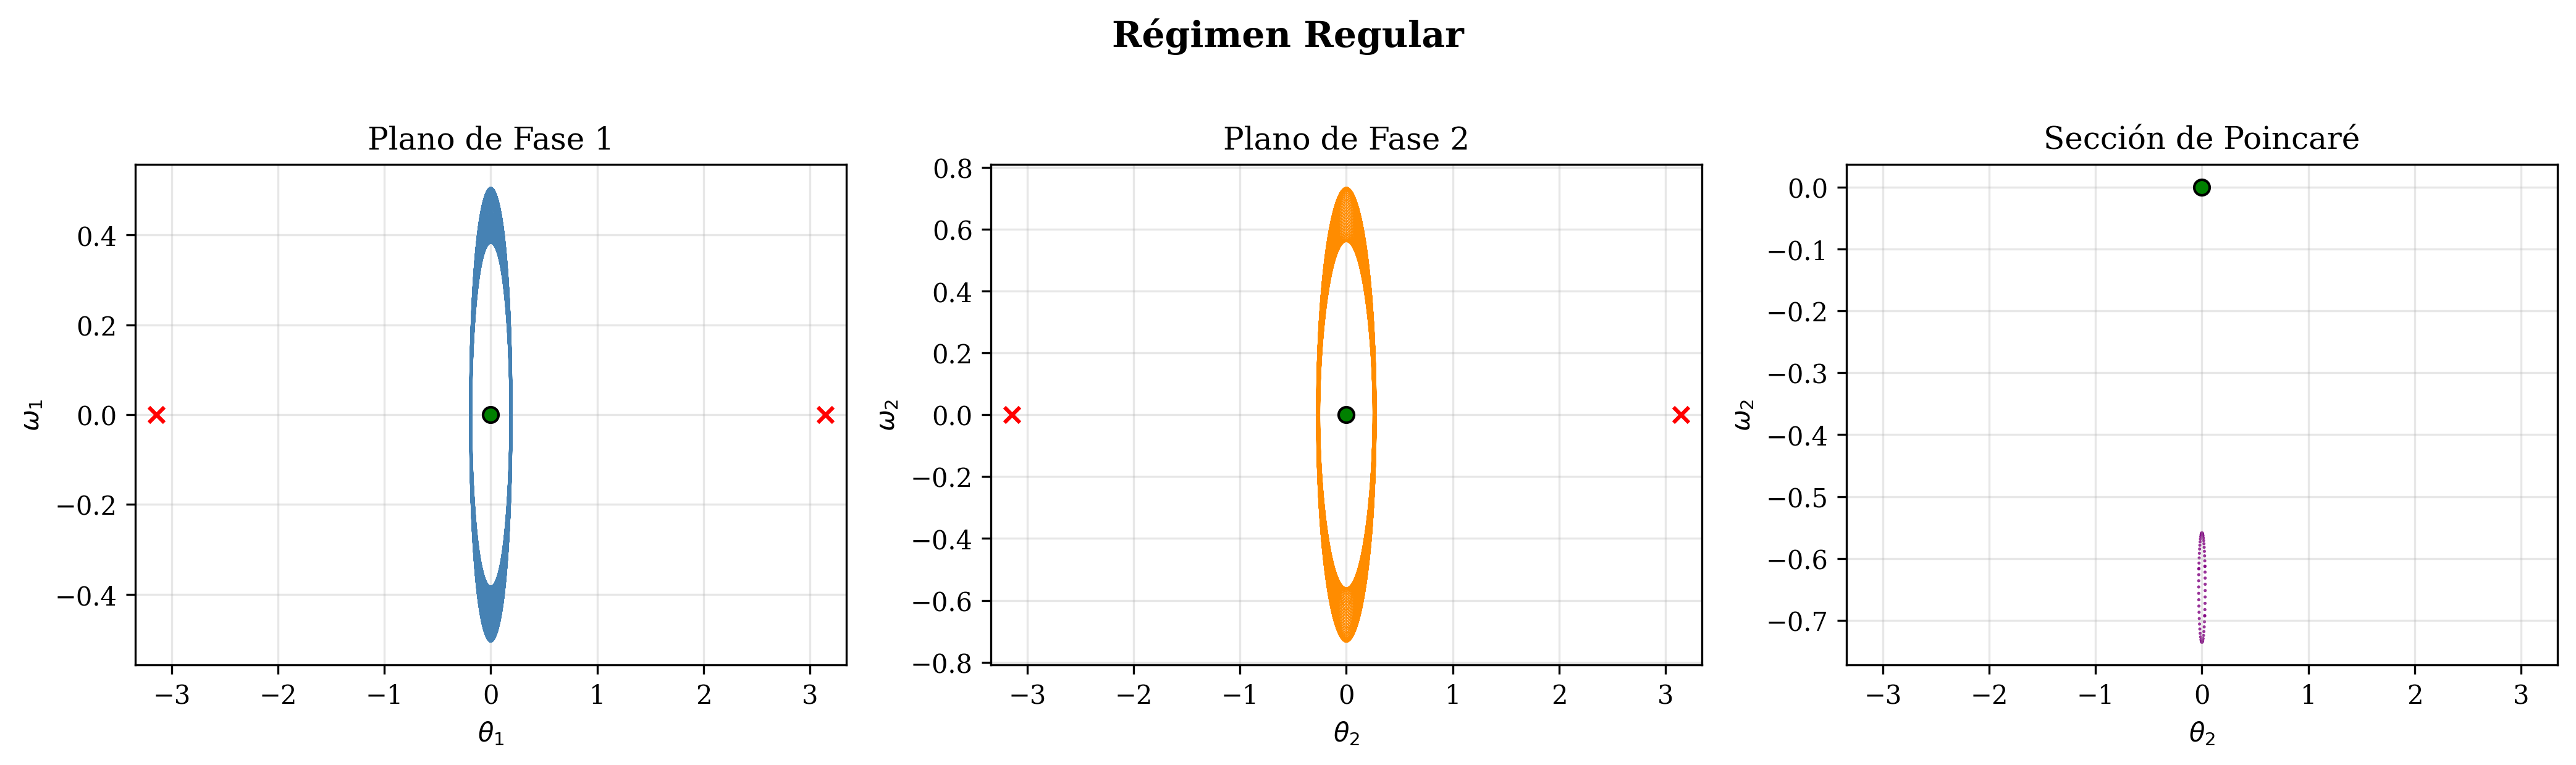
\includegraphics[width=1\textwidth]{regimen_regular.png}
    \caption{Dinámica regular ($E < E_{c1}$). Las trayectorias carecen de la energía suficiente para alcanzar los puntos de silla y quedan confinadas a oscilaciones alrededor del centro $(0,0)$. La sección de Poincaré proyecta un toro KAM perfectamente preservado.}
    \label{fig:regular}
\end{figure}

Como predice el modelo de potencial, al no tocar los puntos críticos, el flujo es regular y no presenta homoclinicidad. Los retratos de fase muestran órbitas cerradas homotópicas a un punto. En la sección de Poincaré (Figura \ref{fig:regular}), la iteración del mapeo forma curvas invariantes cerradas. El desplazamiento del centro de la elipse a lo largo del eje de las ordenadas en ciertas condiciones indica un estado de rotación cuasi-periódica pura, sin bifurcación hacia el caos.

\subsubsection*{Caso 2: Intersección de Variedades Invariantes (Dinámica Caótica)}

Con la condición inicial $x_0 = [\pi-0.05, \pi-0.05, 0.0, 0.0]^T$, el sistema adquiere una energía $E \approx 58 \text{ J}$, la cual se aproxima al máximo inestable ($E \approx E_{c3}$).

\begin{figure}[htbp]
    \centering
    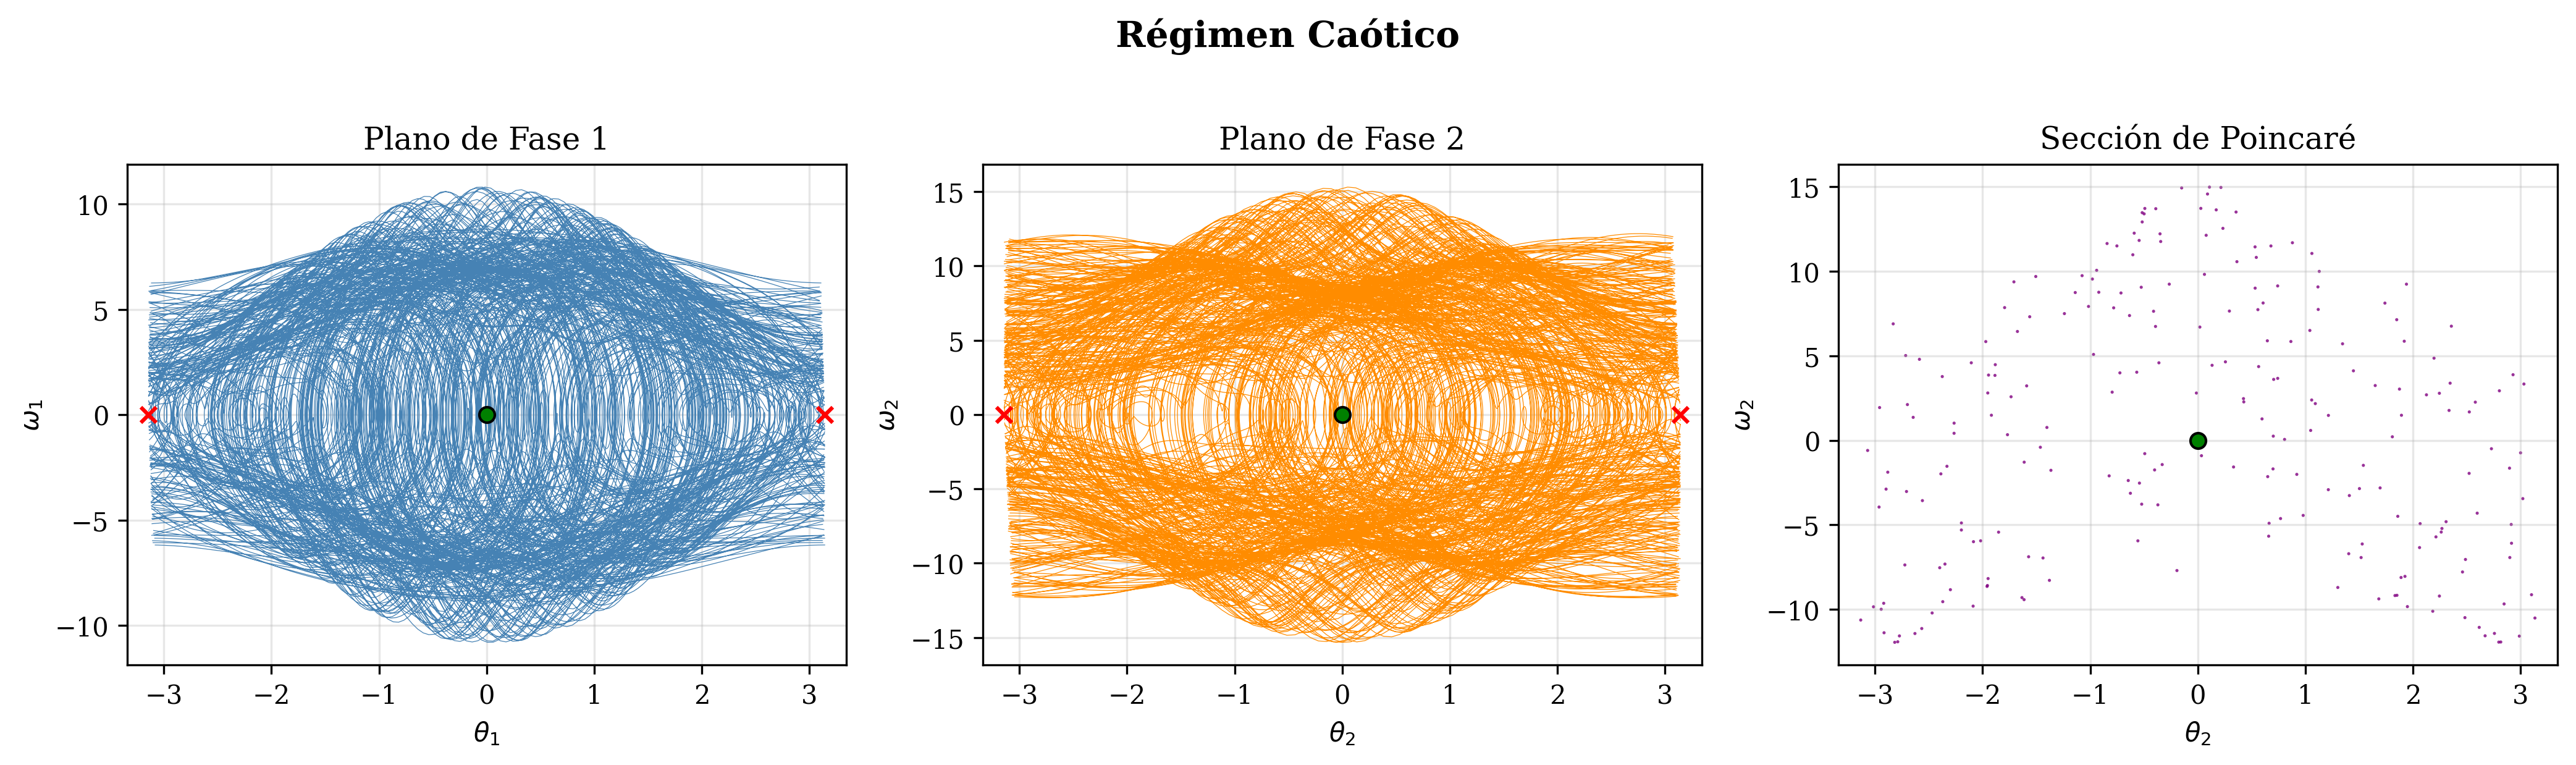
\includegraphics[width=1\textwidth]{regimen_caotico.png}
    \caption{Dinámica caótica ($E > E_{c2}$). El sistema transita repetidamente cerca de los puntos de silla, destruyendo las curvas invariantes y generando una dispersión topológica o ``polvo fractal'' en el mapa de Poincaré.}
    \label{fig:caos}
\end{figure}

En este nivel energético (Figura \ref{fig:caos}), el sistema supera los umbrales de bifurcación $E_{c1}$ y $E_{c2}$. El flujo evoluciona aproximándose iterativamente a las vecindades de los puntos de silla. Al ser un sistema Hamiltoniano que preserva volumen en el espacio de fases, la trayectoria no es atraída a los equilibrios, sino que es repelida a través de las variedades inestables $W^u$. La intersección transversal entre las variedades estables ($W^s$) e inestables ($W^u$) induce una dinámica homoclínica. Numéricamente, esto se visualiza en la sección de Poincaré como un llenado denso de puntos carente de curvas unidimensionales, demostrando la destrucción de la integrabilidad del sistema y la sensibilidad exponencial característica del caos determinista.

\section{Conclusiones}

El presente trabajo demostró la riqueza topológica del péndulo doble al integrar el análisis dinámico cualitativo con la simulación numérica. A través del formalismo lagrangiano y el estudio del espacio de fases, se identificaron exitosamente los estados de equilibrio y los umbrales críticos de energía ($E_{c1}$, $E_{c2}$) que rigen la estabilidad del sistema.

La implementación computacional validó con precisión las predicciones teóricas. Mediante la reducción dimensional del mapa de Poincaré, se logró visualizar la persistencia de los toros KAM en regímenes de baja energía (dinámica cuasi-periódica regular). Asimismo, al incrementar la energía, se constató empíricamente la ruptura de estas curvas invariantes y la emergencia de ``polvo fractal'', evidenciando el enredo homoclínico y la transición hacia el caos determinista. En síntesis, la complementariedad entre el marco analítico y las herramientas numéricas resultó indispensable para comprender la profunda complejidad e impredecibilidad de este sistema.
\end{document}